%!TEX root = spores.tex

\section{\Acf*{SPOR}}%
\label{SPOR}%
\label{sec:SPOR}%
\label{sec:message_passing}%

Say that Alice wants to send a message \(m\) to Bob.
Bob creates a reply header using \(\CreateReply\) and gives the output to Alice 
over an out-of-band channel\footnote{%
  There can be many reasons for this and many ways to solve it.
  \Eg \(m\) might be unavailable at the time.
  Signal creates \ac{DH} exponents in advance (before \(m\) is known) and 
  publishes on the Signal servers, so Alice would fetch one of Bob's when she 
  has a message to send.
  We will treat this in more detail later.
}.
At a later point, Alice attaches a message \(m\) to the reply header using 
\(\UseReply\), creates a forward header using \(\CreateFwd\) with the prepared 
reply header as parameter.
Then she sends this packet to the first node, which processes it using 
\(\ProcessHeader\).
The node will then process the header and in turn forward the packet to the 
next node.
At some point the message will reach Bob who identifies the message as the 
one expected to come from Alice.
%(This process is illustrated in \cref{fig:file-transfer}.)
Now we will focus on two problems that Alice and Bob have:
first, how Alice and Bob choose the nodes that they provide to \(\CreateReply\) 
and \(\CreateFwd\);
second, how Alice and Bob can reduce the use of the out-of-band channel.

%\begin{figure}
%  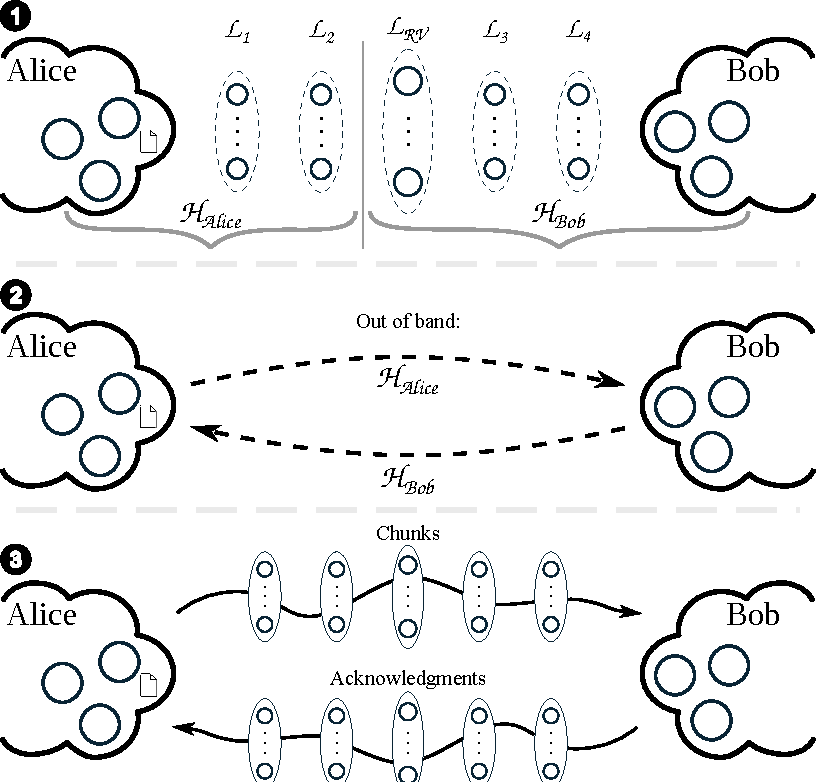
\includegraphics[width=\linewidth]{figures/file_transfer_v2.pdf}
%  \caption{\label{fig:file-transfer}%
%    A schematic of Alice and Bob sending a message using \name.
%    \ding{182} illustrates the layer of the headers that Alice and Bob create.
%    In \ding{183}, Alice and Bob exchange the headers out-of-band.
%    In \ding{184}, Alice and Bob use two \ac{SPOR} routes, one for messages and 
%    one for acknowledgements.
%  }
%\end{figure}

\subsection{Selecting nodes}

There are many uses of SphinxES, many criteria that can be used to select the 
nodes in each layer.
We will now describe the protocol~\(\SPOR\), which uses SphinxES to transfer 
messages from a source to a destination.
It chooses nodes to optimize for availability of each layer.
It also chooses them uniformly randomly from the entire set of 
devices~\(\devices\).

\((d, \pk_d, a_d)\gets \GetNode\): We assume that there exists an 
algorithm~\(\GetNode\) which returns a tuple \((d, \pk_d, a_d)\) of one 
selected node, where
\begin{itemize}
  \item \(d\) is the node's identifier (address);
  \item \(\pk_d\) is the node's public key;
  \item \(a_d\gets \avail(d)\) is the availability of device~\(d\), where the 
    function~\(\avail\colon \devices\to \interval{0}{1}\) maps a device to its 
    availability (0 is always offline, 1 is always online).
\end{itemize}
We note that the function~\(\avail\) does note necessarily have to return the 
exact availability of \(d\), \eg it can provide \(k\)-anonymity by mapping the 
\(d\)'s availability to the closest of some predefined availability values, 
such as \(\{0.25, 0.5, 0.75, 1\}\).

The \(\GetNode\) algorithm can be instantiated using \eg
Octopus~\cite{Octopus}, which would yield a near uniform distribution of nodes 
under adversarial conditions.
Another instantiation would be Tor's authoritative directory servers.
However, exactly how the \(\GetNode\) algorithm is implemented is not our 
concern at the moment.

Now we can construct the layers of Bob's reply block that Alice can use to send 
him a message.
We provide the algorithm \(\CreateLayers\), which populates the layers~\(L_0, 
\dotsc, L_{\nu-1}\) that Bob must provide to \(\CreateReply\).
(Bob will create \(L_\nu\) himself by filling it with his devices.)

\((L_0, \dotsc, L_{\nu-1}) \gets \CreateLayers\):
The algorithm first makes \(\nu\cdot w_L\) queries to \(\GetNode\) to get 
enough nodes to fill all layers.
These nodes are distributed across all layers~\(L_i\), for \(0\leq i < \nu\), 
to maximize the availability~\[
  a_{L_i} = 1 - \prod_{d\in L_i} (1-a_d)
\] of every layer (or equivalently, minimizing the risk that every node in a 
layer is offline at the same time) while keeping \(|L_i| = w_L\).

\subsection{Reducing the use of the out-of-band channel}

It is desirable for Alice and Bob to use out-of-band communication as little as 
possible.
To do this, we define \ac{SPOR} to let the first part of the payload to be a 
reply header that the recipient can use to reply.
